\documentclass[twocolumn]{article}
\usepackage[width=17cm,height=22cm]{geometry}
\usepackage[english]{babel}
\usepackage[utf8]{inputenc}
\usepackage{fancyvrb}
\usepackage{authblk}
\usepackage{hyperref}
\usepackage{outlines}
\usepackage{graphicx}
\usepackage{color}
\DeclareGraphicsExtensions{.pdf,.png,.jpg}

\newtheorem{theorem}{Théorème}
\definecolor{vthierry}{RGB}{80,0,120}\newcommand{\vthierry}[1]{{\color{vthierry}{#1}}}
\definecolor{thalita}{RGB}{51, 153, 255}\newcommand{\thalita}[1]{{\color{thalita}{#1}}}

%%%%%%%%%%%%%%%%%%%%%%%%%%%%%%%%%%%%%%%%%%%%%%%%%%%%%%%%%%%%%%%%%%%%%
%% AUTHOR GUIDELINES
%% See https://www.frontiersin.org/about/author-guidelines 
%%%%%%%%%%%%%%%%%%%%%%%%%%%%%%%%%%%%%%%%%%%%%%%%%%%%%%%%%%%%%%%%%%%%%%
\bibliographystyle{alpha}
\title{Not-so-big data deep learning} 
\author[1]{Thalita F. Drumond}
\author[1]{Thierry Vi\'eville}
\author[1]{Fr\'ed\'eric Alexandre}
\affil[1]{Mnemosyne team, INRIA Bordeaux}
\begin{document}
\maketitle

\begin{abstract}
  bla bla.
\end{abstract}
\medskip

\noindent\textbf{Keywords}: Deep-learning, Not-so-big data, Meta learning, Representation learning, Transfer learning.

\section*{Introduction}

Organisation proposée pour l'intro:
\begin{outline}[enumerate]
\1 avènement du DL et du big data avec impact important en machine learning
\1  faire revue de papiers de deep-learning avec plein de variantes par rapport a l architecture de LeCun utilisé p bcp de tâches dont utilisé pour la vision
\2 review de la jungle des CNN : \cite{Srinivas2016Taxonomy}
\2 LeNet-5 \cite{Lecun1998Gradient}
\2 Boom with AlexNet  that used a CNN architecture that not only won the Imagenet contest, but got a 12\% drop in the state-of-the-art error rate \cite{Krizhevsky2012Imagenet}. In the subsequent session of the contest, CNN based architectures kept scoring the best rankings: ZF net \cite{Zeiler2014Visualizing} and Overfeat net in 2013\cite{Sermanet2013Overfeat}, VGG net \cite{Simonyan2015Very},  GoogLeNet \cite{Szegedy2014Going} in 2014, residual nets in \cite{He2016Deep}.
\1  annoncer au début qu'on va traiter de manière generale de DL et qu'on va examplify with problems in vision and mostly with convolutional networks mais nos arguments seront plus généraux et pourront s'appliquer à d'autres architectures de DL et d'autres domaines d'application, except when we make it explicit; et pour le cas particulier de la vision on va faire positioning wrt tasks
(object (localization|detection)|scene (parsing|classification)) of interest here
\1 dans ces approches data driven, les datas sont bien sur essentielles et il faut se poser des questions sur la qualité et la quantité des data à disposition; en particulier, pour la plupart des pbs réalistes, on n'a pas tant d'exemples que ça; ça peut poser pb p appliquer le DL dans ces conditions; en fait, plutôt not so big data que very few data; pour donner un ordre de grandeur, parler de dizaines ou centaines ou milliers d'ex; Il faudra aussi préciser ça plus bas dans le texte en spécifiant les différents types de contraintes; real-time learning on doit réagir rapidement; active learning on a un nb limité d'ex mais on peut les choisir; transfer learning on se sert d'autres domaines de connaissances; si le recueil d'ex est long ou coute cher, on va être limité à un nb mais sans pouvoir les choisir, etc.
   \2 extremely small dataset problems:  one-shot learning (one example per class) and zero-shot learning (...) \cite[presents them as transfer learning tasks]{Goodfellow2016Representation}. Intermediate: few-shot learning (k examples per class),
\1 Considering this short state of the art, the aim of this paper is to conduct an experimental work NOT in order to study yet another architecture dedicated to one of the generic tasks reviewed here, but INSTEAD (to be reformulated) to study how to optimize the architecture, with a main objective: obtain reasonable performances on not-so-big data set.
\1 It is a major issue in many situations where either parsimonious data sets only are available, or real-time constraints yield the need to provide a best-effort estimation with the data available at a given time.
\1 Regarding the challenge to consider not-so-big data set, the issue of micro-data learning, in a extreme situation, is addressed by rather different methods \cite{Mouret2016Micro}, though the three basic precepts (i) actively search about which is the most relevant data to consider (active learning), (ii) exploit every bit of information (detailed learning), (ii) use as much as possible a-priori data (generative learning) are taken into account in the our approach.
\1 From the previous review we can make explicit several levers to deal with not-so-big data sets in deep learning architectures: announce and define the list of sections below; en faisant référence à la figure qui énonce les différentes étapes de mise en oeuvre de DL; 
d'une part travailler sur le corpus (en augmentant artificiellement le nb d'ex ou en les choisisant ou autres actions sur input space) ou travailler sur les caractéristiques du modèle particularly parameters (faire une meilleure initialisation ou diminuer leur nb), architecture (implique aussi changement nb param mais autres sujets possibles plus sur implication fonctionnelle), error function, metric, etc.) 
\1 differentiate between list of possible ways and what will be considered experimentally here et indiquer qu'on pourra aussi faire référence à l'apport de la bio-inspiration.  (fin de l'intro)
\end{outline}

Considering the specifications in \cite{Bengio2007Scaling}, the main issue here is to do the best out of a bounded number of samples. This includes good estimation performances (thus good generalization). Taking into account the not-so-many data constraint, and having the no-free-lunch theorem in mind\footnote{The no-free-lunch theorem for machine learning states that if an algorithm performs well on a certain class of problems, then it necessarily pays for that with degraded performance on the set of all remaining problems, up to performing no better than blind search if considering ``all'' possible problems.}, we target methods dedicated to a not-entirely-general data set, for not-all-tasks but a specific small subset, when not one.
More specifically, here we will focus on semantic segmentation.

We also are not going to tackle the challenge of reducing computations during training and during recognition, but will favor sub-optimal methods and architectures allowing to optimize the previous requirements. We will thus not address real-time issues, except the on-demand paradigm aspect (i.e., being able to make available the current best result at any time).

The amount of human labor necessary to tailor the algorithm to the task is also going to be considered, but not in the sense of \cite{Bengio2007Scaling}: The goal of requiring the smallest possible amount of additional hand-specified knowledge for each specific task is not an issue here, but a potential strength. Indeed, specifying explicit prior knowledge built into the model before training is going to be a lever to gain efficiency in this context. Nonetheless implicit opaque adjustment through engineering design is going to be avoided, attempting not to manually adjust architecture (e.g. number of layers) or meta-parameters (e.g. learning rate). Thanks to many existing methods we are going to integrate such meta-parameters in the learning parameters mechanism itself, in order to optimize the estimation performances.



How to deal with a task specific and data class specific not-so-big data set is thus the main issue of this paper. We are going to discuss in details each issue and propose concretely an dedicated estimation method, referred as Task Fine Data estimation (TFD-estimation) as make explicit in the sequel.



\section{Multiplying data} 
% augmenting our "sampling" of the input space
In this section we discuss several strategies that in one way or another, try to cope with the small data problem directly at the data level: by making it not so small. 
% Consider the scenario leading to the small data problem
The constraint of learning over a small dataset might emerge from different practical situations. 

% If labeling is the problem - semi-supervised
Labeling sometimes is the major bottleneck (due to time or human expertise availability constraints). In that case, if extra unlabeled data samples are available, then a semi-supervised strategy allows to exploit a larger number of examples. Another alternative is to simplify the labeling task as much as possible. For instance, for a scene semantic segmentation task, if having a fully pixel-wise labeled image is too expensive, we can consider having only bounding boxes roughly circling the main objects of the scene.

We might be retrieving labeled data points in real-time, slowly growing our dataset with selected examples. In that case, we have full interest in optimizing our retrieval strategy along the learning process, a technique(?) referred to as active learning \cite{Settles2010Active}. \thalita{ It is a variant of semi-supervised learning, in which we choose to be labeled only examples that are highly expected to improve learning.

MENTION HERE: 
\cite{Woodward2016Active} Active one-shot learning
}

% When dimensionality is so huge that any amount of data becomes small
Regardless of the reason leading to a small dataset, high dimensional input spaces are a frequently related issue. Data from neuroimaging studies are a good example on this matter. Due to constraints in the number of participants and access to equipment, usually few trials are made, leading to small datasets. If we are to use the raw data directly, each example has millions of voxels, leading to a poorly sampled input space, regardless of how many volunteers participate in the study. In such situations dimensionality reduction and feature extraction methods (such as ICA\cite{Hyvarinen2000Independent}, PCA, etc.) are often necessary steps.

(\cite{Plis2014Deep} comment on that, then try to validate the use of deep models for neuroimaging data)

(Comment on regular sampling and sampling on regions of interest eg frontier points in SVM. navigating the input space needs a metric)

% le miracle de la multiplication des données XD
\thalita{Artificially augmenting the dataset with synthetic data is another trick of the trade often used to train deep learning models. Data augmentation is a general guide line that can be equally used with shallow feature extractions methods and yield analogous boosts in performance, even though still inferior to deep models \cite{Chatfield2014Return}.}
The simplest case is to add some sort of noise to you input data. Here we use noise in a large sense: not only additive noise but also relevant distortions and transformations \cite{Poggio1992Recognition, Simard2003Best}. Note that these transformations have to make sense in the input data domain, and are usually derived from domain specific symmetries. This can be easily exemplified in the image domain: an image classifier ideally should output the same labels for a mirrored image or a slightly rotated one. Thus, these are appropriate transformations to expand the input dataset. 
Being easy to implement, this strategy has been widely used in the image recognition domain, from LeNet \cite{Lecun1998Gradient} in 1998 and still today. 

Unfortunately finding such transformation can be less obvious in other domains. With this in mind, \cite{Devries2017Dataset} proposed to augment data directly at the feature space, created through a sequence autoencoder.




Synthetic data can also be obtained by combining original data (REF), or by learning a generative model (REF). These approaches imply an explicit modeling of the data, which will be further discussed in the Data Model section.


To be added in the section:
% commenting out what has been treated in the text above
\begin{outline}
% \1 What is the problems we want to consider with the input space? are we only constrained by a limited number of examples (eg: real-time), but we can choose and define a strategy of data selection ? (cf Active Learning, tech report \cite{Settles2010Active}). Are we given a limited corpus with no choice of example possible and we must cope with this? Is only labeling the costly process (because time or resource of expertise difficult to find) but we can have many non labeled (or poorly labeled) data (pixel labeling more expensive than defining regions of interest) ?
\1 consider the general problem of having a large input space with few samples inside: which strategies ? 
% \2 one strategy can be to decrease the size of the input space (dimensionality reduction mais cf section nb parameters plutot concernée par ça); 
\2 wonder about uniform sampling versus sampling in regions of interest, for example where errors have been done before, or sampling at the border between regions (cf dancing boys). but this possible if we can choose examples, cf active learning.
% \1 increase artificially the number of data by adding noise (but need to define a metric and the kind of noise to be added).
\1 another classical problem with set of examples in the input spaces is to share them between learning, test and validation corpus and to organize learning protocole accordingly (eg: cross-validation); this part will be considered in section Learning Protocole but here,  consider that the idea of epoch, iteration of epochs until convergence etc is already related to the fact that data are limited, else we would work online, we would have a new example every time (not really a dataset)... In this respect, at the frontiers between multiplication of data and adaptation of the learning protocoles, we could consider the idea of adapting the learning protocole online as a function of the kind of error (for example to remove the outliers from the learning or present more often examples yielding more errors; cf also links to boosting or to mixture of experts) EXPERIMENTS COULD BE DONE HERE... (voir aussi si cette histoire d'adapter le learning protocole ne serait pas mieux dans la section Learning protocoles...); voir aussi l'idée de créer de nouveaux exemples comme combinaison d'anciens...
\1 As far as data is concerned, the simple idea is to wash-out the rather small data-set, i.e., experiment to which extents re-using several times a data sub-set until the final-convergence yields a negligible bias on the final estimation or not. Since the learning data is embedded in a metric space (i.e. we can compute a "distance" between samples), it is possible to propose data selection heuristics (e.g. depending on the task, select samples that properly cover the whole data space, or samples close to the frontier between two categories in a classification or detection task, since such samples are more crucial for the discrimination). With this choice, there is the known drawback that the data being no more randomly sampled, the learning algorithm has a biased estimation of the sample probability distribution, thus a worst generalization capability. This is still valuable for constrained data set.

\1 discuss link with hippocampus and general/specific cases
\end{outline}

\vthierry{In order to take these considerations into account, we need a proper metric on the data set, whereas estimating the such a metric is an indirect goal of the tasks considered here (see the discussion on data model, below). A step further, in order to apply sophisticated selections on the data set, we need to subdivide it in several subsets as with meta-learning heuristics \cite{Bergstra2012Random}, which is a bit contradictory with need to to use as much data as possible for estimation and set. }


\section{Initial conditions and transfer learning}
% Taking a good start
% parameter space again, but this time not on its dimensionality. The model keeps its complexity, we only start "closer" to an interesting region.

Neural network models are non-convex optimization problems with multiple local minima. A different minima is reached at every run, depending on the initial state of the model parameters. It makes sense to consider prior domain knowledge to determine suitable initial conditions, possibly leading to a better solution. 
Careful initialization has always been a concern when training neural networks, and particularly important for deeper networks, where traditional normally-distributed random initialization of weights performs poorly. \cite{Glorot2010Understanding} analyze this problem and suggest a commonly-used heuristic initialization method that brings faster convergence.
If computational power is available, an exploratory strategy can be taken, with multiple initializations tried in parallel, keeping only the most promising ones. However for large deep models, such approaches become prohibitive.

\thalita{In the image recognition domain, the popularization of CNN models and the ImageNet competition lead to a situation where all the main models are implemented and have their trained weights available for download. Initially crafted for the 1000-classes prediction task, they started being reused for other tasks and datasets, with minor adaptations, leading to successful results \cite{Razavian2014Cnn}. These supervised pre-training strategies came to be known as transfer learning. }

Transfer learning aims to improve a model by transferring information from a previously trained model from another domain \cite{Weiss2016Survey}. One of the forms to do it is to use pre-trained features, transferring the weights of the first layers of a network trained for a task A to a network that will perform a task B. Learning task B will train mostly the parameters of the final layers, maybe fine-tuning the ones transfered from task A. This form of transfer learning can be seen as a way start training on better initial conditions, and stands on the assumption that tasks A and B share some low-level features. This seems to be particularly true for visual tasks, where reusing part of a network trained with general domain data gives surprising results. The transferring may go as far as using the previous model as a feature extractor for a subsequent classifier, with the original weights not being adjusted at all during training (eg: OverFeat + SVM \cite{Razavian2014Cnn}). How far the transfered layers should be kept untouched or fine-tuned is related to the size of the target dataset, as demonstrated in \cite{Soekhoe2016Impact}. Their overall conclusion is: the smaller the target dataset is, the more rigid the transfer should be.

\thalita{Transfer learning usually comprises an architectural adaptation side, either because of a difference in the number of classes in the dataset, or because the prediction task is inherently different. In \cite{Zeiler2014Visualizing}, their CNN model was originally targeted at ImageNet, but they also tested it in other datasets by redesigning and retraining the final layers to match the new number of classes. In the case of a different task, changing might be more extreme. As an example let us consider semantic segmentation. In this task, where all pixels of an image have to be individually classified, it is common to reuse pre-trained architectures but changing the  final fully connected layers to convolutional ones \cite{Long2015Fully}. For such task, the multiple pooling layers have a major drawback of reducing resolution and limiting the precision of the boundaries arising from the final pixel-class prediction. With that in mind, different adaptations have been proposed such as skip-pooling connections \cite{Long2015Fully}, dilated (à trous) convolution \cite{Chen2016Deeplab,Yu2016Multi} and even the use of a decoding architechture \cite{Noh2016Learning,Badrinarayanan2015Segnet}.}

EXPERIMENTS POSSIBLE HERE
Transfer learning could be experimented from other data sets or from a priori basic filters (derived from statistics on natural images\cite{Torralba2003Statistics}) or even from adjustable weights following a variational approach. 

\thalita{HMAX-type models \cite{Serre2005Object,Theriault2011Hmaxs}  inspired in the works of Hubel and Wiesel \cite{Hubel1959Receptive} use fixed gabor filters on first layer to mimic edge and orientation detection present in cortex V1. Before AlexNet sucess on ImageNet the setting of these first layer filters used to be more discussed as a critical issue \cite{Jarrett2009What}. Now it is usually thought they can be learned from data (if there is enough) or that the knowledge can be transfered from a large dataset to a small one. However when developing new architectures, having a better knowledge of what to put in the first filters could avoid a long pre-training step. Besides, if the target dataset has too different statistics than those of the source dataset (as is the case with natural and manufactured scenes \cite{Torralba2003Statistics}), transferring filters might not be as effective.}

\cite{Riesenhuber1999Hierarchical}


 


\section {Restrict parameter space}
\thalita{
% reducing parameter space dimensionality
% Reduction of dimensionality also mentioned elsewhere should be discussed here. -> no in data model.
Restricting the parameter space of a model --- eventually reducing its number of parameters --- is an important strategy to avoid overfitting, which is particularly relevant when dealing with not-so-big datasets. 

\paragraph*{Weight-sharing} 
In comparison to fully connected deep architechtures, convolutional layers act as a locally connected layer with shared weights. These two characteristics --- local connections and weight sharing --- effectively reduce the number of parameters and can be considered in other applications that could benefit from the translation equivariance proper to this connectivity pattern. Analogously, other weight-sharing schemes could be imagined tackling other desired invariances.(WOULD BE NICE TO FIND AN EXAMPLE) 
}

\thalita{
\paragraph*{Weights as functions} 
Instead of assuming scaler values, the entries of a weight matrix can follow a family of suitable functions that will enforce certain invariances } (eg. weights as a function of an angle or a scale-factor in relation with rotation or zoom invariance) and symetries (e.g. isotropic diffusion, or linear combination of horizontal and vertical diffusion) proper to the application domain. 
Another track is (by analogy with the kernel trick) to consider linear combination of predefined local operators, each operator being known as efficient to extract some cue. This includes also non-linear combination, as for instance, considering normalized gain control. (the idea here would be to go toward something more generic thanks to these combinations and consequently less 'expensive'). 

\thalita{
\paragraph*{Weight regularization} 
Imposing a regularization constraint over weights in a network is one of the restriction forms. In machine learning in general, deep architectures included, L2 regularization on the network weights (also called weight decay) is commonly used \cite{Simonyan2015Very,He2016Deep}. However, some argue that such regularization is not so relevant in early convolutional layers because they are more involved in feature extraction than on prediction (NEED REF OTHER THAN FORUM DISCUSSIONS). Conversely, since features and prediction are learned together, regularization could be helping to learn features better adapted to the subsequent classifier layers (not entirely clear to me).

Less wide-spread in deep supervised models is the use of L1 regularization to induce sparseness. One may naturally think of it for sparse individual connections, but it is also possible to induce sparsity in the number of channel connections between convolution layers, implicitly learning architechtural meta-parameters together with network weights (further discussed in section arch).  
In unsupervised models it is more common to have sparsity constraints aiming at a sparse final representation -- sparse coding. Such approaches will be discussed in the next section (?).

This idea of sparse connections is present in two training techniques that can be seen as a form of regularization --- Dropout \cite{Srivastava2014Dropout} and DropConnect\cite{Wan2013Regularization} --- where at every step a certain percentage of connections (or channel connections) is set to 0, cutting them out from output generation and also from gradient backpropagation. Although all connections participate at evaluation time, dropout leads to fewer connections effectively coding each prediction.
}
% Beyond the issues reviewed in the previous paragraphs, we are facing both a parameter adjustment problem (finding the best weights values) and a meta-parameter adjustment problem: adjusting the convolution mask sizes, considering the use of parameterized predefined weight profiles versus unconstrained weight values, image resolution at a given layer, counting the number of channels to take into account.


%% THALITA: UNCOMMENT IN CASE IT GOES BACK TO BEING AN EXPERIMENTAL PAPER:
% Here the proposal is to integrate such meta-parameter adjustment within the parameter adjustment, as developed in \cite{Drumond2017From}.

% -In order this huge accumulation of heterogeneous channels to be tractable, we are going to extensively use strong sparse estimation. We should not only apply a ${\cal L}_1$ criterion on the related parameters but introduce either more drastic approximation of the ${\cal L}_0$, (e.g., ${\cal L}_p, p < 1$ or more efficient methods [LASSO ? Greedy pursuit ? Convex relaxation ? Heuristic such as reset on the N smallest values ? => a voir ensemble selon ce que TensorFlow sait faire ou peut implementer]).


TBD in this section:
\begin{itemize}
\item Cite Mallat and wavelets, as another example for having few parameters for a good power of expression if the 'fonction mère' is well chosen... Or mention also the idea of a variational approach. 
\item discuss link with biological data about visual cortex, coding of masks of columns of orientation. 
\end{itemize}



\begin{figure*}
\label{diagram}
\centering
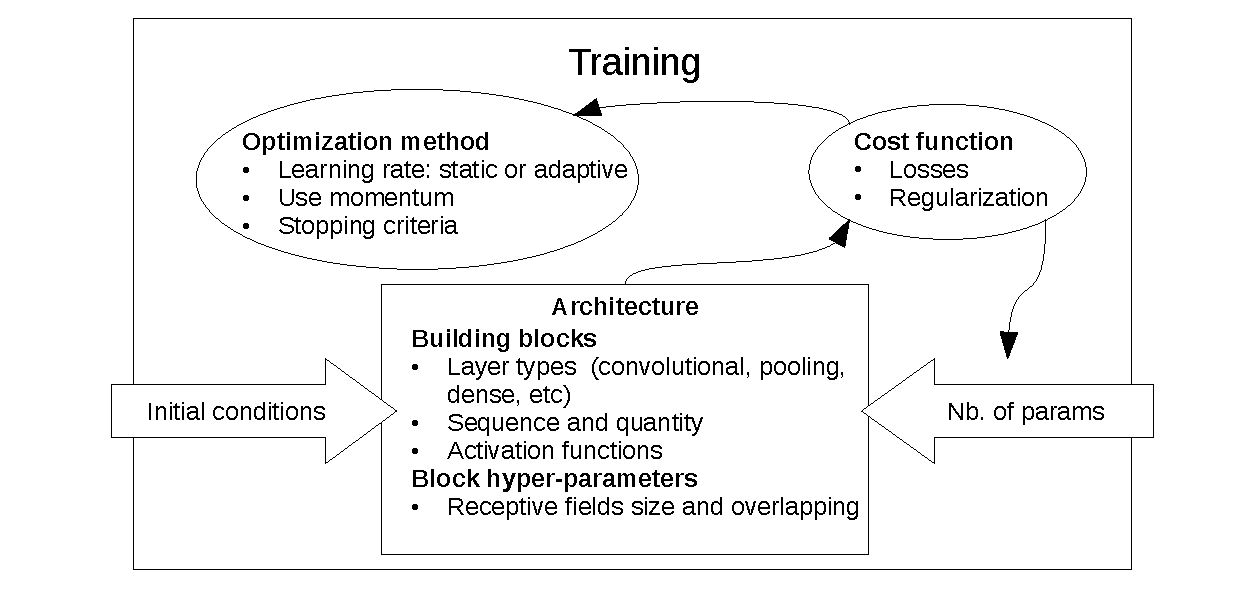
\includegraphics[width=0.8\textwidth]{img/diagram}
\caption{Schematic representation of the different element of deep-learning approach related to the not-so-big data issue. See text for details.}
\end{figure*}







\section{Unsupervised data model}

\begin{outline}
\1  representation learning \cite{Bengio2012Representation,Goodfellow2016Representation}
\\ - specify the task-specific prior knowledge in the structure of a graphical model by explicitly representing important intermediate features and concepts through latent variables whose functional dependency on observed variables is hard-wired
\2Transfer learning also comprises unsupervised pre-training and is related to the general goal of learning representations.
\1 try to model the data distribution, uncovering the underlying factors. They might assume a hierarchical structure.
\1 related to disentangling underlying factors, learning the data manifold (dimensionality reduction)
\1 learn invariants (related to weight sharing too) 
\2 unsupervised eg \cite{Anselmi2016Unsupervised}
\2 spatial transformer nets : explicitly allows the spatial manipulation of data within the network, resulting in models which learn invariants \cite{Jaderberg2015Spatial}
\1 sparsity or other structure 
\1 comment on adversarial training? Generative adversarial networks

\end{outline}
% representation learning

\vthierry{Here we want to model data in the following sense: given a specific task, e.g. classification, and a data set, how to infer a suitable model ? The key aspect is that it is equivalent to infer a metric. Let us clarify this point.

Classification or data clustering, for instance, (but also other task such as recommendation, i.e., finding data points closed to a given one), all relate on the qualitative simple idea of being able to compute the distance between data points (e.g., is a test sample closer to a given category prototype of support vector than others). This is also true for dimensional reduction, since it the data manifold is ultimately defined by the underlying Riemannian metric. This is still true for disentangling underlying factors or explicit invariant, since it is on one hand related to finding the manifold on which these factors stand, and on the other hand projecting the data samples on a manifold where each point correspond to an invariant value. 

The general observation is that given a data point ${\bf x}_0$ and its transformation via the deep-learning layers ${\bf x}_l, 0 < l \leq L$ a metric is induced $d({\bf x}, {\bf x}') = \sum_{l=0}^L |{\bf x}_l - {\bf x}'_l|_l$ for some metric, e.g. ${\cal L}_d$. This means that before adjusting the weight for a given task, we may adjust the weights in order to have a suitable metric, and perform a transfer learning from this first weight estimation to the task specific weight estimation, with the hope that the initial weight value is pertinent. 

Here we are going to consider the case where the learning data is exact (e.g., no misclassification) and maximize the [JE SUIS PAS A COURS D IDEES (imposing i.i.d. of the samples by maximizing entropy, positionning of the samples with margin in suitable part of the space) MAIS JE VEUX BIEN REBOUCLER AVEC VOUS AVANT]
}

\section{Optimization}

Training of deep models poses particular difficulties: local minima, saddle points and plateaus, vanishing or exploding gradients, long and difficult convergence (LIST GOES ON ADD REFS OTHER THAN BOOK CHAPTER \cite{Goodfellow2016Optimization}). Multiple strategies have been proposed to tackle these issues, including the use of improved versions of the SGD algorithm, batch normalization \cite{Sergey2015Batch}, use of relu non-linearities  \cite{Krizhevsky2012Imagenet, He2015Delving}. 
We know little about how these strategies influence learning from small datasets.


\paragraph*{Loss function} When solving classification problems, using a log-loss function (cross-entropy) is a widespread practice, and few works explore the use of other functions \cite{Janocha2017Loss}. Some loss functions might be more robust to small datasets where classes are under-represented. (TO BE DEVELOPPED FURTHER)
Besides the main loss function, other terms in the loss function might be of interest depending on the task performed. For instance image reconstruction models might benefit from a total variation regularization over the network outputs \cite{Jin2016Deep}. 

\paragraph*{Learning protocol} principled guidance of the optimization procedure can be relevant for extracting the maximum out of a small dataset. In \cite{Ravi2017Optimization}, a meta-learning approach is taken where a LSTM model helps decide the parameter updates by training and evaluating multiple CNN models. 


TBD 
\begin{outline}
\1 multi-task learning
\1 - \cite{Le2011optimization}


\1 séparer loss et regularizer: plutot une approche supervisée p le loss et non supervisée p la regularisation

\1  se définir une distance pour calculer l'erreur en sortie (cf regularisation mais aussi faux positifs ou negatifs)  
 
\1 Concerning error function, cf also the principle of regularization which might be useful, including the idea to have close internal representations for examples with the same label (and conversely). 

\1 EXPERIMENT POSSIBLE HERE: Cost function using cross-entropy should be more costly than using distance L1 or L2

\1 With few data, possible to give an answer with better arguments/explanation. 

\1 Regularization can be used to obtain sparseness or implement total variation in hidden layer

\1 - plutôt appliquer un critère à marge que bêtement mettre une SVM en couche finale, ceci de façon à optimiser plus profondément les poids pour obtenir une meilleure classification.
\1 - voir à utiliser des soft-max en concurrence avec de la SVM ou du FC-perceptron.
\end{outline}

\section{Architectures}
%choix du Lego; 
% double issue = which blocks + block metaparams
%[WHAT ELSE ? stride of convolution fields, pooling type, size of pooling windows (fixed or adaptive), with or without overlapping, type of non-linearity] 
\thalita{
Architechtural choices can have an important impact on the learning capability of the model and thus can be a lever for enhancing learning out of small datasets. Whether supervised pre-training over large datasets is possible or not (section transfer learning), one might want to consider whether and how to best adapt a deep architecture for his own application.
}

\thalita{
Tuning the deep architecture itself is a double issue. On one hand, given an architecture and its building-blocks, there are many hyper-parameters to be tuned such as the number of units, size of the convolution fields, number of stacked homogeneous layers. 
On the other hand, blocks of a certain type (like convolutional, pooling or dropout \cite{Hinton2012Improving} layers) can be qualitatively added or removed, allowing us to adjust the optimal processing capability. 

There have been some attempts at developing automated hyper-parameter search strategies other than manual or grid-searching \cite{Bergstra2012Random, Goodfellow2016Practical}. Works proposing new architectures usually test a few different configurations (eg. VGG\cite{Simonyan2015Very} and ResNet\cite{He2016Deep} test different network depths), although the extent of the exploration stays rather limited due to computational and time constraints. Many hyper-parameters remain rather unexplored, following filter and layer sizes used in previous works. 

Given a base architecture as a starting point, some works have tried to adapt the architecture by iterating a network pruning step and a re-training step. This idea of optimizing network connections a posteriori is not new \cite{Lecun1990Optimal,Hassibi1993Optimal}, but just recently has been applied to deep architectures. It is usually  aimed at compressing models for faster evaluation, but in some cases it can bring performance improvements.
In \cite{Han2015Learning}, they train once to get a connectivity pattern by thresholding out low weighted connections. Then they re-train to actually learn weights, iterating between pruning and re-training.

MENTION HERE:

Evolutionary architecture search \cite{Real2017Large}.

Reinforcement learning for architecture design \cite{Zoph2016Neural}.


Instead of meta-optimizing architectural parameters, they can be parameterized in order to be included in the learning process. One way of doing so is to include a sparsity criteria over a particular architectural feature. For example, \cite{Wen2016Learning} propose a structured sparsity scheme (using a group-LASSO criteria) to learn sparse structures filer-wise, channel-wise, filter shape-wise, and layer depth-wise. They apply their regularization scheme to LeNet, AlexNet and ResNet, obtaining significant reduction in all of these parameters, with no loss (and sometimes improvement) of accuracy. As with most sparse-structuring approaches, their work focused on speeding-up computations, although it also hints that performance can be improved by co-learning weights and architectures.  

}
\cite{Iandola2016Squeezenet}



Inception\cite{Szegedy2014Going,Szegedy2016Inception,Szegedy2016Rethinking}).



TBD:
\begin{outline}
\1 Shortcuts with residual networks
	\2 Proposition of the residual building block \cite{He2016Deep}. Won 1st prize on ImageNet detection, localization and COCO segmentation. Performs well in different visual tasks - authors believe its generic and should apply to other domains.
    \2 can be seen as a way of shutting off some layers : a step in the direction of the "complete acyclic" network?
	\2 Other examples: Inception res net \cite{Szegedy2016Inception}, Wide res nets\cite{Zagoruyko2016Wide}
   \1 Equivalently, considering a maximal architecture with the lattice of all possible modules connected, qualitatively changing the architecture corresponds to open or close some short-cuts, i.e. add modulatory parameters on all connection weights between an inter-layer connection. With this trick, qualitatively tune the architecture itself, falls down to a meta-parameter sparse optimization (i.e. considering continuous values, but with a preference to set value to zero, in order to reduce the number of degree of freedom of the estimator). 
Here we only consider feed-forward architectures (thus an acyclic graph with a supremum and infimum), while recurrent architectures are also considered in a parallel work within a well-defined framework, but beyond the scope of this work. Except for the special case of an attentional feed-back or using the feed-back of errors or considering the RBM. 
\1 For simple architectures without combinatorial explosion, the different possibilities can be enumerated, choosing the best. 

\1 (Here, links could possibly be proposed with biological inspiration concerning the pulvinar and also concerning attentional processes coming with feedback; need to describe how attention is selected, for example linked to prediction of error. )

\1 All together, we propose to not simply put a lot of modules together and rely on deep-learning to manage to cope with the whole estimation problem, but introduce a-priori information via parameter constraints (including structural parameters).

\1  ajouter la possibilité de connections multiplicatives entre couches ou de memory carrousel pour augmenter la non-linéarité du processus.

\end{outline}

\bibliography{thalita,future}

\end{document}
